\documentclass[a4paper, 12pt]{article}
\usepackage[T2A,T1]{fontenc}
\usepackage[utf8]{inputenc}
\usepackage[english, russian]{babel}
\usepackage{graphicx}
\usepackage[hcentering, bindingoffset = 10mm, left = 15 mm, right = 15 mm, top=25mm]{geometry}
\usepackage{multirow}
\usepackage{lipsum}
\usepackage{amsmath, amstext}
\usepackage{siunitx}
\usepackage{subcaption}
\usepackage{wrapfig}
\usepackage{adjustbox}
\usepackage{enumerate, indentfirst, float}
\usepackage{capt-of, svg}

\newenvironment{bottompar}{\par\vspace*{\fill}}{\clearpage}
 
\begin{document}
\begin{titlepage}

\newcommand{\HRule}{\rule{\linewidth}{0.5mm}} % Defines a new command for the horizontal lines, change thickness here

\center % Center everything on the page
 
%----------------------------------------------------------------------------------------
%	HEADING SECTIONS
%----------------------------------------------------------------------------------------

\textsc{\LARGE Московский Физико-Технический Институт}\\[1,5cm] % Name of your university/college
\textsc{\Large Кафедра общей физики}\\[0.5cm] % Major heading such as course name
\textsc{\large Лабораторная работа \textnumero  3.4.2}\\[0.5cm] % Minor heading such as course title

%----------------------------------------------------------------------------------------
%	TITLE SECTION
%----------------------------------------------------------------------------------------

\HRule
\\[0.4cm]
{ \huge \bfseries Закон Кюри-Вейсса}
\\[0.2cm] % Title of your document
\HRule
\\[1.5cm]


 
%----------------------------------------------------------------------------------------
%	AUTHOR SECTION
%----------------------------------------------------------------------------------------

\begin{minipage}{0.4\textwidth}
	\begin{flushleft} \large
		\emph{Автор:}\\
		Ришат \textsc{Исхаков} % Your name
	\end{flushleft}
\end{minipage}
~
\begin{minipage}{0.4\textwidth}
	\begin{flushright} \large
		\emph{Преподаватель:} \\
		Александр Александрович \textsc{Казимиров} % Supervisor's Name
	\end{flushright}
\end{minipage}

\begin{bottompar}
	\begin{center}
		\includegraphics[width = 80 mm]{logo.jpg}
	\end{center}
	{\large \today}

\end{bottompar}
\vfill % Fill the rest of the page with whitespace

\end{titlepage}

\section{Цель работы}

Изучение температурной зависимости магнитной восприимчивости ферромагнетика выше точки Кюри.

Внешнее магнитное поле ориентирует магнитные моменты, которые в отсутствии поля располагались в пространстве хаотичным образом. Ферромагнитные вещества, которые при понижении температуры становятся парамагнитными должны подчиняться закону Кюри-Вейсса: $$ \chi = \dfrac{1}{T-\Theta_p}, $$ где 
$\Theta_p$- температура, близкая к температуре Кюри. 

В нашей работе мы изучали температурную зависимость $\chi(T)$ гадолиния при температурах выше точки Кюри. Для гадолиния точка Кюри лежит в пределах комнатных температур.

\section{Экспериментальная установка}

\begin{figure}[H]
\centering
	 \includegraphics[width = 0.8 \textwidth]{Scheme}
\caption{Схема экспериментальной установки}

\textit{1 - Катушка с образцом, 2 - стеклянный сосуд с трансформаторным маслом, 3 - вода в термостате, 4 - ртутный термометр, 5 - термостат}
\end{figure}
Параметры установки: $k = 24 \text{град/мВ}$ ;
$\tau_0 = 8.252 \text{мкс}$

\section{Работа и измерения}

Нашей задачей является проверка выполнения закона Кюри-Вейсса. Зная, что при изменении температуры должна меняться магнитная восприимчивость гадолиния, а, следовательно, и самоиндукция катушка, будем замерять период колебания $\tau$ в колебательном контуре в зависимости от температуры вещества $T$. Разность между температурой в термостате $T_\text{изм.}$ и реальной температурой вещества можно оценить с помощью термопары $\Delta U$ и коэффициента установки $k$. Проверим выполнение соотношения: 
$$ \dfrac{1}{\chi} \sim (T- \Theta_p) \sim \dfrac{1}{(\tau^2-\tau_0^2)}, $$ где $\tau_0$ период колебаний в отсутствии образца.

\begin{table}[H]
\centering
\resizebox{\textwidth}{!}{%
\begin{tabular}{|c|c|c|c|c|c|c|c|c|c|c|c|c|c|c|c|c|c|c|}
\hline
$T_\text{изм.}, \SI{}{\degreeCelsius}$                                          & 14.75 & 15.00 & 16.52 & 17.15 & 18.20 & 19.17 & 20.11 & 21.10 & 22.08 & 23.06 & 24.06 & 26.06 & 28.04 & 30.01 & 32.01 & 34.00 & 35.99 & 39.97 \\ \hline
$\Delta U, \text{мВ}$                                                    & -0.02 & -0.02 & -0.02 & -0.02 & -0.02 & -0.01 & -0.02 & -0.02 & -0.02 & -0.01 & -0.02 & -0.01 & -0.02 & -0.01 & -0.02 & -0.02 & -0.02 & -0.02 \\ \hline
$T, \SI{}{\degreeCelsius}$                                                    & 14.39 & 15.00 & 16.52 & 17.15 & 18.20 & 19.17 & 20.11 & 21.10 & 22.08 & 23.06 & 24.06 & 26.06 & 28.04 & 30.01 & 32.01 & 34.00 & 35.99 & 39.97 \\ \hline
$\tau, \text{мкс}$                                               & 10.07 & 10.06 & 9.94  & 9.88  & 9.74  & 9.57  & 9.40  & 9.19  & 9.01  & 8.84  & 8.74  & 8.61  & 8.54  & 8.49  & 8.46  & 8.44  & 8.42  & 8.39  \\ \hline
$\tau^2 -\tau_0^2, \text{мкс}^2 $& 33.26 & 33.04 & 30.65 & 29.44 & 26.85 & 23.51 & 20.28 & 16.43 & 13.16 & 10.00 & 8.29  & 5.95  & 4.78  & 3.98  & 3.46  & 3.05  & 2.73  & 2.28  \\ \hline
$1/(\tau^2 -\tau_0^2), 1/\text{мкс}^2 $ & 0.03  & 0.03  & 0.03  & 0.03  & 0.04  & 0.04  & 0.05  & 0.06  & 0.08  & 0.10  & 0.12  & 0.17  & 0.21  & 0.25  & 0.29  & 0.33  & 0.37  & 0.44  \\ \hline
 $\Delta(1/(\tau^2 -\tau_0^2), 1/\text{нс}^2 )$ & 0.09  & 0.09  & 0.11  & 0.11  & 0.14  & 0.17  & 0.23  & 0.34  & 0.52  & 0.88  & 1.27  & 2.43  & 3.73  & 5.35  & 7.07  & 9.05  & 11.26 & 16.14 \\ \hline
\end{tabular}%
}
\caption{Данные с установки}
\end{table}

Строим график зависимости $1/(\tau^2 -\tau_0^2) = f(T)$ для определения парамагнитной точки Кюри $\Theta_p$ для гадолиния и $\tau^2 -\tau_0^2 = f(T)$ для проверки формулы.

\begin{figure}[H]
\centering
	 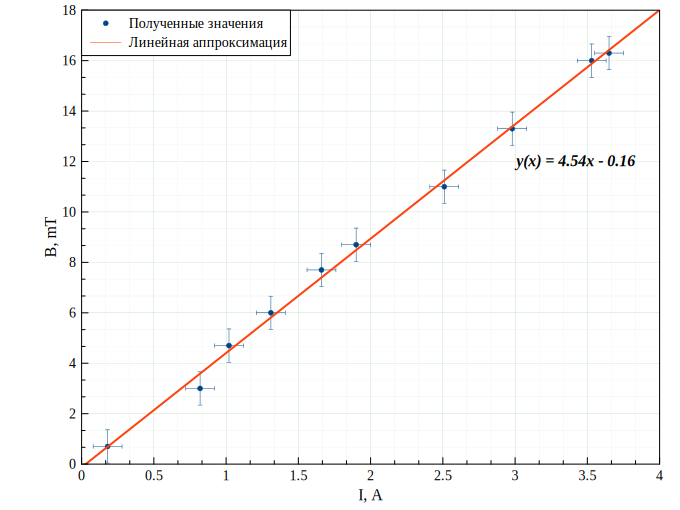
\includegraphics[width = 0.8 \textwidth]{Graph1}
\caption{Зависимость $1/(\tau^2 -\tau_0^2) = f(T)$}
\end{figure}

\begin{figure}[H]
\centering
	 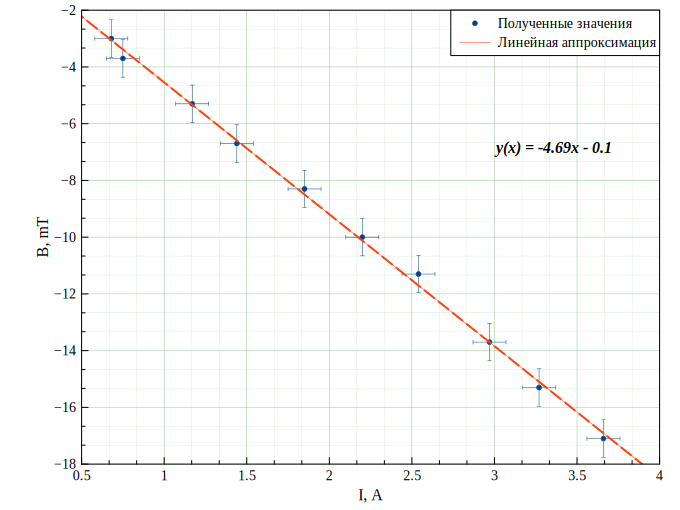
\includegraphics[width = 0.8 \textwidth]{Graph2}
\caption{Зависимость $\tau^2 -\tau_0^2 = f(T)$}
\end{figure}

По уравнению прямой оценим значение парамагнитной точки Кюри $\Theta_p$ для гадолиния: $$\Theta_p = 17.68 \pm 4.28 \SI{}\degreeCelsius$$

Табличное значение: $\SI{16}\degreeCelsius$

\section{Вывод}

Полученное значение с учетом погрешности измерения соответствует действительности. Возможные причины погрешности измерения состоят в разнице температур между термостатом и гадолинием, несмотря на то, что это учитывается при расчете. Погрешность на частотомере очень мала.



\end{document}